\documentclass{sig-alternate-05-2015}
\usepackage{tabu}
\usepackage{multirow}
\usepackage{graphicx}
\usepackage{float}

\makeatletter
\def\@copyrightspace{\relax}
\makeatother
\begin{document}

% Copyright
\setcopyright{acmcopyright}

\title{Web Economics: Individual Report}

\numberofauthors{1}
\author{
\alignauthor
Devin Kuokka\\
      \affaddr{Group 09}\\
      \affaddr{COMPM041: Spring 2017 Coursework}\\
      \affaddr{Affiliate Student, Computer Science}\\
      \affaddr{University College London}\\
      \email{devin.kuokka.16@ucl.ac.uk}
}
\maketitle

\section{Introduction}
In an increasingly digital society, online advertising has become imperative to the success of businesses, and placing an ad in the right place at the right time, can have substantial financial impact on companies.  The improvement of technology and the increased competition have popularized real-time bidding systems: an auction system that allows advertisers to bid on certain ad spaces given information about the user, page, and context (Figure X). Beyond simply winning the ad, however, it is crucial for advertisers to maximize the number of ads they purchase that are \emph{actually} clicked on by users. Thus, developing an effective bidding strategy that maximizes the click through rate (CTR) while operating under a constrained budget, can have significant positive influence on companies competitive performance in the digital sphere. I attempt to achieve this goal by: (1) exploring the log of over 2.5 million bid requests, (2) developing a strong learning algorithm (hereon referred to as model) that generates a pCTR for a given bid request, and (3) instantiating an effective bidding strategy that maximizes the purchase of clicked bids and minimizes the purchase of non-clicked bids, all under the constraint of a budget.

The approach discussed in this paper is based off the preliminary results and pitfalls of a linear bidding strategy, which are discussed in detail in Section \ref{approach}.  While the new model and bidding strategy did manage to win all 226 clicked bids in the validation set, I was unable to improve the pCTR.  Thus, my attempt to increase the \textit{f1\_score}, discussed in section \ref{approach}, was unsuccessful.

\section{Related Work}
Due to the nature of real data, class imbalance has become a popular topic in the machine learning community. Haibo He and Edwardo A. Garcia do a wonderful job of thoroughly discussing the class imbalance in \textit{Learning from Imbalanced Data}. He and Garcia cover everything from sampling methods, to learning algorithms, to metrics. The comprehensive study is one of few that focuses on a theoretical approach to the problem of class imbalance rather than case studies or specific algorithms. One area where the paper lacks is the discussion of feature selection with imbalanced data.  Maldonado, Weber, and Famili discuss backwards elimination, with each succession holding out more features that are determined via a balanced loss function generated on an independent subset of the data \cite{featureSelection}. While both \cite{imbalanced} and \cite{featureSelection} discuss precision, recall, and f1 (discussed in later sections) as potential performance metrics, neither have expanded on their potential uses in other steps of the learning process.

\section{Data Exploration} \label{dataExploration}

\begin{table}[h]
\centering
\begin{tabu} { X[l] x[c] x[l] x[c]}
 \hline
 \multirow{2}{4em}{Attribute} & \multirow{2}{4em}{Unique Entries} & \multirow{2}{4em}{Included?} & \multirow{2}{4em}{One Hot Encoded?} \\
 \\
 \hline
 Click & 2 & --- & ---\\
 Weekday & 7 & Yes & Yes\\
 Hour & 24 & Altered & Yes\\
 Bid ID & 2,697,738 & No & ---\\
 Log Type & 1 & No & ---\\
 User ID & 2,591,064 & No & ---\\
 User Agent & 39 & Altered & Yes\\
 IP & 515,530 & No & ---\\
 Region & 35 & Yes & Yes\\
 City & 370 & Yes & Yes\\
 Ad Exchange & 5 & Yes & Yes\\
 Domain & 24,087 & Yes & Yes\\
 URL & 833,453 & No & ---\\
 URL ID & 1 & No & ---\\
 Slot ID & 55,983 & Yes & Yes\\
 Slot Height & 21 & Altered & No\\
 Slot Width & 14 & Altered & No\\
 Slot Visibility & 11 & Yes & Yes\\
 Slot Format & 4 & Yes & Yes\\
 Slot Price & 284 & Yes & No\\
 Creative & 130 & Yes & Yes\\
 Bid Price & 8 & --- & ---\\
 Pay Price & 301 & --- & ---\\
 Key Page & 19 & Yes & Yes\\
 Advertiser & 8 & --- & ---\\
 User Tag & 814,364 & No & ---\\
 \hline
\end{tabu}
\caption{Dataset Features Details}
\label{features}
\end{table}

My training dataset includes the bid request information for over 2.5 million impressions. This log provides information about the user, ad, page, and context for each bid request. Table \ref{features} provides details of each attribute.

\begin{table}[h!]
\centering
\begin{tabular}{l c c }
 \hline
 Total Impressions & 2,679,738 \\
 Clicks & 2,034 \\
 Total Cost & 216,496.24 \\
 CTR & 0.0754\% \\
 Avg CMP & 106.44 \\
 Avg CPC & 80.25 \\
 \hline
\end{tabular}
\caption{Basic Dataset Performance Metrics}
\label{dataMetrics}
\end{table}

As demonstrated by Table \ref{dataMetrics}, this data is highly imbalanced: for every click, there are roughly 1,317 non-clicks.  This imbalance plays a fundamental role in the development of the model discussed in section \ref{approach}.

Unfortunately, due to the anonymity of the data---i.e. attributes, such as region, are given as integer values rather than as interpretable strings---I could not measure the correlations between each attribute and click occurrence.

Based upon the non-linear modeling strategy discussed in \cite{nonlinear}, the bidding strategy is dependent upon the distribution of the ad prices (denoted by payprice in the dataset).  Figure \ref{payPriceDist} shows the distribution of all ad prices within the dataset, while Figures \ref{payPriceDistClicked} and \ref{payPriceDistNonClicked} show the ad prices distributions for clicks and non-clicks, respectively. How these figures impact the bidding strategy used will be discussed in Section \ref{biddingStrategy}.

\begin{figure}
   \begin{minipage}{0.5\textwidth}
     \centering
     \includegraphics[width=1\linewidth]{payPriceDist.png}
     \caption{Distribution of Pay Prices for all Bid Requests}
     \label{payPriceDist}
   \end{minipage}\hfill
   \begin {minipage}{0.5\textwidth}
     \centering
     \includegraphics[width=1\textwidth]{payPriceDistClicked.png}
     \caption{Distribution of Pay Prices for all Clicked Bid Requests}
     \label{payPriceDistClicked}
   \end{minipage}
   \begin {minipage}{0.5\textwidth}
     \centering
     \includegraphics[width=1\textwidth]{payPriceDistNonClicked.png}
     \caption{Distribution of Pay Prices for all Non-Clicked Bid Requests}
     \label{payPriceDistNonClicked}
   \end{minipage}
\end{figure}

\section{Individual  Approach \& Results} \label{approach}
Preliminary work with the original model revealed four areas in which potential improvement could be found: (1) increasing precision, recall, and the F1 Score, (2) improving feature selection, (3) applying a different learning algorithm, and (4) learning on a different performance metric.

Precision, or Specificity, is defined as TP/(TP+FP), where TP is true positives and FP are false positives, and is the model's ability to not label a negative bid as positive.  Recall, or Sensitivity, is defined as TP/(TP+FN), where TP is true positives and FN is false negatives, and is the model's ability to correctly identify all positive bids. The F1 Score is given by 2*(precision*recall)/(precision+recall), and is the weighted average of precision and recall. As discussed in \cite{imbalanced}, precision, recall, and F1 are better metrics to examine when dealing with imbalanced data, as they are not as sensitive to the imbalance as accuracy, the typical measure used.

\subsection{Feature Selection}

Due the severe class imbalance, identifying which attributes are most indicative of a click is essential to developing a strong pCTR predictor, and later bid price.  As shown in Table \ref{features}, a majority of the attributes were categorical, and included in the feature set.  Attributes were excluded if there were too many unique values or two few; in both cases, the predicative power of the attribute is diminished. Additionally, those with too many values were all categorical and would have to be one-hot-encoded, which would dramatically increase the feature space and slow down the learning time; the additional benefit of their predictive power does not out weight the runtime cost. As indicated in Table \ref{features}, I used one-hot encoding to incorporate the categorical variables into the feature space.  Attributes that were marked as \textit{altered} were stratified into new features, shown in Figure \ref{stratifiedFeatures}, to increase their predictive power.

\begin{figure}[h]
 \centering
 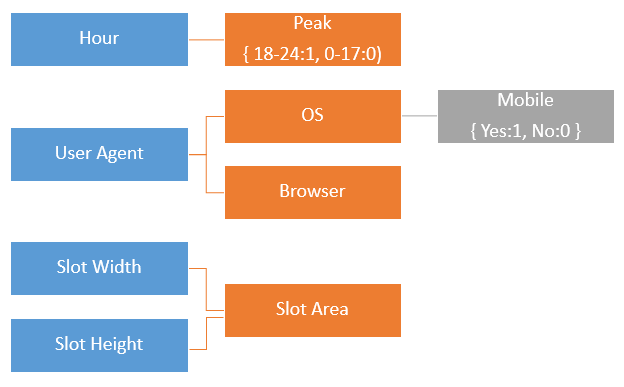
\includegraphics[width=1\linewidth]{modifiedFeatures.png}
 \caption{Stratification of Select Features}
 \label{stratifiedFeatures}
\end{figure}

I defined peak hours to be from 16-24 because during non-peak hours, when individuals are either sleeping, working, going to school, or running errands, people have more free time to peruse ads and explore online. I separated User Agent into OS and Browser to increase the generalization across bids, thereby increasing the predicative power. From here, I separated OS into mobile or computer, as whether people click ads on phones versus computers is likely more telling than simply what OS they are using.  Finally, I combined slot width and slot height into slot area because the overall size of the ad is more indicative of its being clicked on than its shape.

\subsection{Preprocessing Data}
To tackle the data imbalance problem and to increase runtime, I took a random undersample from the majority class, producing training data that had 5 non-clicks for every click (as opposed to the original 1,317).  I chose 5 because in \cite{zeroMult}, King and Zeng recommend an undersampling ratio between two and five times that of the minority class for the optimal trade-off between data imbalance and explanatory variable predictability strength. Additionally, my cross validation metric preforms better with more data, so I opted for the maximum of the two to five range.

Utilizing a confusion matrix (Table \ref{confusionMatrix}) on the original model showed that a large portion of my budget was being spent on false positives, or bids that the model said would be clicked, but were not.

\begin{table}[h!]
\centering
\begin{tabular}{ | c | c | c |}
 \hline
 & Predicted Non-Click & Predicted Click \\
 \hline
 True Non-Click & True Negative & False Positive \\
 \hline
 True Click & False Negative & True Positive \\
 \hline
\end{tabular}
\caption{Confusion Matrix}
\label{confusionMatrix}
\end{table}

These false positives contribute to a lower CTR and increased expenditure.  To decrease the number of false positives, I employed a new feature selection method: \textit{selectFPR}, which selects all the features with p-values below the provided alpha (0.01), as determined by an FPR test, or False Positive Test, thereby reducing the number of false positives that my model predicts.

\subsection{Learning Model}
I elected to use \textit{logisticregressionCV} (hereon referred to as LRCV) as my learning algorithm because it enables more customization than other classification algorithms, and uses parameters that theoretically solve many of my issues.

Since I am undersampling the majority class, I lose a significant portion of the training data, which reduces the effectiveness of my model. LRCV, however, uses \textit{StratifedKFold} cross validation, which preserves the class percentages and helps prevent overfitting; this form of cross validation allows me to undersample a larger number of non-clicks, more accurately representing the full dataset, and increasing the total training data via both more raw data and cross validation.

Furthermore, LRCV allows me to specify what metric to use as the cross validation criteria. I selected the \textit{f1\_score} metric, as it factors in both precision and recall, and should provide better results than the default \textit{accuracy\_score}, as discussed in Section \ref{approach}.

Finally, LRCV allows me to apply a penalty (\textit{l1}), which is helpful with feature selection, overfitting prevention, and combating data imbalance.

\subsection{Bidding Strategy} \label{biddingStrategy}
The distributions shown in Figures \ref{payPriceDist}, \ref{payPriceDistClicked}, and \ref{payPriceDistNonClicked} are right skewed, indicating that the non-linear bidding strategy discussed in \cite{nonlinear} should be used---with a high concentration of ads at the lower end of the price spectrum, it is ideal to prioritize winning the lower priced bids.  The non-linear bidding equation provided in \cite{nonlinear}:
\begin{equation}
bidPrice = \sqrt{\frac{\textit{c}}{\lambda}\theta + \textit{c}^{2}} - \textit{c} \tag{\textit{(1)}}
\end{equation}
where \textit{c} is a constant and $\lambda$ is the Lagrangian multiplier, works such that increasing the unit bid for low bids increases the winning rate more than it does at high bids.

\subsection{Parameter Tuning}
There are two parameters I can tune in the non-linear bidding strategy: \textit{c} and $\lambda$.  To determine the optimal trade off, I first made the assumption, based on equation \textit{(1)}, that \textit{c} is similar to a base bid. Therefore, I set \textit{c} to the average CPC found in Section \ref{dataExploration}: 80.23.  From here, I tuned $\lambda$.  Since a majority of the bids that are clicked are under 120 RMB (\ref{payPriceDistClicked}), I set the base bid for the median click probability (roughly 0.48) provided from the model.  Thus, I determined a starting $\lambda$ as 0.001.  These results did not produce optimal CTR's or clicks, so from here I simply tuned $\lambda$ until I reached the results in section \ref{results}.  The ultimate values for $\lambda$ and \textit{c} were 0.000212 and 80.25, respectively.

\subsubsection{Results} \label{results}
Given a budget of 25,000 CNY, my model and bidding strategy produced the results below:

\begin{table}[h!]
\centering
\begin{tabular}{l c c }
 \hline
 CTR & 0.0754\% \\
 Clicks & 226 \\
 Total Cost & 24,045.22 \\
 Avg CMP & 80.22 \\
 Avg CPC & 106.39 \\
 \hline
\end{tabular}
\caption{Individual Model and Bidding Strategy Results}
\label{results}
\end{table}
\end{subsection}

\section{Conclusion}

Unfortunately the results did not reflect an improvement in the \textit{f1\_score} as I had hoped. While I was able to capture all the bids, a CTR score of 0.00075 is no better than that of the training data, discussed in Section \ref{dataExploration}.  An improvement in the CTR would have indicated a reduction in the number of bids on non-clicked bids, or false positives.  I suspect the problem lies with the learning model, rather than with the non-linear bidding strategy: if there were a clear distinction between the pCTR's of clicked versus non-clked bids, then CTR would increase because the model can accuratly predict a click probability for each bid, that is then used in the non-linear bidding strategy to determine a bid price. Additonally, excessive tuning of \textit{c} and $\lambda$ saw CTR improvement. Based upon the research regarding performance metrics, I believe that using a different learning algorithm, such as decision trees or random forests, would produce better results with the same non-linear bidding strategy.

Moving forward, I would explore cost-based machine learning algorithms discussed in \cite{imbalanced} \cite{featureSelection} \cite{costSensative} \cite{costBalance}.  The general approach is to develop a cost matrix in the same format as a confusion matrix (Table \ref{confusionMatrix}), giving different weights to each of the four possibilities.  The learning algorithm will then optimize the performance, taking these weights into account.  In respect to my data, where there was a significant cost to misclassifying non-clicks, but also a need to correctly identify clicks.  Allocating costs more specific to the individual advertiser or problem could produce better results.  Beyond improving the model, I would also have liked to explore some other non-linear bidding models, specifically ones that use the remaining budget as a parameter.

My function in the group was to primarily to theorize, research, and test different approaches to improve the pCTR prediction model, and select a non-linear bidding strategy.  I was critical in understanding and implement ORTB1 from \cite{nonlinear}, and helped to optimize the final model.  I adapted the code, produced by Michael, and tested out new theories to maximize my groups output relative to time spent.  Stelios optimized the constant and random bid strategies, as well as drafted a majority of the final report. Michael produced all the code, and helped optimize the final bidding strategy.

\begin{thebibliography}{5}

\bibitem{nonlinear}
Weinan Zhang, Shuai Yuan, and Jun Wang.
Optimal real-time bidding for display advertising. In
\textit{Proceedings of the 20th ACM SIGKDD international conference on Knowledge discovery and data mining, pages 1077–-1086.}
ACM, 2014.

\bibitem{imbalanced}
Haibo He, and Edwardo A. Garcia.
Learning from Imbalanced Data. In
\textit{TRANSACTIONS ON KNOWLEDGE AND DATA ENGINEERING, VOL. 21, NO. 9, pages 1263--1284.}
IEEE, September 2009.

\bibitem{featureSelection}
Sebasti\'oan Maldonado, Richard Weber, and Fazel Famili.
Feature selection for high-dimentional class-imbalanced data sets using Support Vector Machines. In
\textit{Information Sciences, Volume 286, Pages 228--246}.
December 2014.

\bibitem{zeroMult}
Gary King and Langche Zeng.
Logistic Regression in Rare Events Data. In
\textit{Political Analysis, Vol. 9, No.2, pages 137--163}
JSTOR 2001

\bibitem{costSensative}
Charles Elkan.
The Foundations of Cost-Sensitive Learning. In
\textit{Proceedings of the Seventheeth International Joint Conference on Artificial Intelligence}
2001.

\bibitem{costBalance}
Charles X. Ling, and Victor S. Sheng
Cost-Sensitive Learning and the Class Imbalance Problem. In
\textit{Encyclopedia of Machine Learning. C. Sammut (Ed.). Springer}
2008.

\end{thebibliography}

\end{document}
